\documentclass[12pt, titlepage]{article}
\usepackage{float}
\usepackage[normalem]{ulem}
\usepackage{color}
\usepackage{enumitem}
\usepackage{booktabs}
\usepackage{tabularx}
\usepackage{hyperref}
\usepackage{textgreek}
\usepackage{graphicx}
\usepackage{indentfirst}
\graphicspath{{img/}}
\hypersetup{
    colorlinks,
    citecolor=black,
    filecolor=black,
    linkcolor=black,
    urlcolor=blue
}
\usepackage[round]{natbib}

\title{SE 3XA3: Test Report}

\author{Team \#3 - Hextron
		\\ Jason Li lij107
		\\ Yousaf Shaheen shaheeny
		\\ Scott Williams willis12
}

\date{December 6, 2017}


\begin{document}

\maketitle

\pagenumbering{roman}
\tableofcontents
\listoftables


\begin{table}[bp]
\caption{\bf Revision History}
\begin{tabularx}{\textwidth}{p{3cm}p{2cm}X}
\toprule {\bf Date} & {\bf Version} & {\bf Notes}\\
\midrule
December 6th & 1.0 & The final test report, with all traces and test results.\\
\bottomrule
\end{tabularx}
\end{table}

\newpage

\pagenumbering{arabic}

\section{Introduction}
This test report document is formulated to validate the requirements that are found in the standard requirements document (SRS) as well as testing the relationships between the different modules that are labelled in the final revision of the Module Guide (MG). This 

\section{Functional Requirements Evaluation}
The functional requirements that are labelled in our test plan are mainly tested through the use of dynamic testing. The series of automated, dynamic unit testing took great advantage of Unity Test Tools, which are bundled in various versions of the Unity game engine. The unit tests included a modifier that labels them as "UnityTest" with square brackets surrounding them. They serve as coroutines, where yielding provides a great advantage of waiting between different phases of each automated test. \\

In our case, the functional requirements tested were also determined by usability surveys in that end users of different age groups and backgrounds were asked to evaluate the core functionality of the Hextron project made by the development team. They were given surveys with basic questions on feed back and no prior instruction in regards to how to play. The executable game file was sent to the testers and they were instructed to play and return the survey mentioning specifically functions that were not working and to not mention functions that were working as expected. With this testing we knew a function was working for users if nothing is mentioned about it.\\

From the test plan, there were eight vital areas of testing that needed to be determined through a series of either manual or automated tests that were of dynamic nature. The reason for this decision was because simple unit tests outside of run time will not properly verify whether game scenarios have the expected and correct outcome. A summary of the testing is described in the table on the next page.

\begin{center}
    \begin{tabular}{ | l | l | l | p{5cm} |}
    \hline
    Area of Testing & Manual & Automated & Description \\ \hline
    1 & Yes & No & Checks whether or not button traversal to open the game menu is correct \\
    \hline
    2 & Yes & Yes & Checks whether a game object rotates along with the hexagon once it is a child trapezoid \\
    \hline
    3 & Yes & Yes & Verifies that the trapezoid game objects exhibit physics and that it moves towards the center hexagon \\
    \hline
    4 & Yes & No & Validates that the trapezoids scale as it approaches the center hexagon from when it spawns. \\
    \hline
    5 & Yes & Yes & Validates whether points are accumulated depending on if a connection of three similar colored trapezoids of green, yellow, blue or red color occur. \\
    \hline
    6 & Yes & No & Validates whether pressing the P key on a standard keyboard will pause the game. \\
    \hline
    7 & Yes & Yes & Verifies that a rainbow colored trapezoid will destroy all blocks surrounding it. \\
    \hline
    8 & Yes & Yes & Verifies that a black trapezoid will not be destroyed upon a connection of three black trapezoids. \\
    \hline
    \end{tabular}
\end{center}

Based on the information that was gathered from the culmination of both usability testing from various end users and dynamic tests, the requirements outlined from our SRS were validated and achieved. This will be further elaborated on inside of the automated testing portion of the Test Plan document. 

\section{Nonfunctional Requirements Evaluation}

\subsection{Usability \& Performance}

For Hextron, a great tool for determining whether non-functional requirements tied to usability and performance was the creation of a usability survey. \\

This usability survey was formulated by Jason Li, and delivered to people of different age groups and professions in order to get a wide range of data that would fulfill fit criterion. \\

Users were told to mention any aspects of the game in which they thought needed improvement as well as any other topic they themselves thought to be a detriment to playing of the game. \\

\textbf{Bootup test} - Sending the executable game file to users they were asked to play the game. With all of our testers being able to run and boot up the game and no mention of errors on boot up we marked the ability to boot up the game as passed.\\

\textbf{Game Running test} - The game was run by all users in all Windows environments and all testers were able to play the game and try the various function of the game as well with no mention of errors upon running the game.\\

\textbf{Game appearance} - Comments were made on the visual appearance of the game with a common mention of the unique font of the game. However there was mention by users of a visual glitch in stacking of the trapezoid. This bug would cause a misalignment of trapezoids which were stacked but had no effect on the functionality of the game. The test was deemed to pass in visual attractiveness for which the test was intended, but fails in the functional test of block stacking.\\

\textbf{Cultural Validity} - no mention of cultural symbolism or offensive imagery were mentioned, therefore the assumption is made that the program passes cultural validity for the small sample size that we had. It doesn't however pass the test in regards to other countries and large scale audience as testing of that scale was out of our scope.\\

\textbf{Legality Testing} - A question was present in asking the similarities of our program to Hextris.io but It was disclaimed that the program was built in a non-profit educational background. Additionally the Hextris program was built with a GPLV3.\\
	
\section{Comparison to Existing Implementation}	

    When comparing to existing implementations before automated, unit testing took place, most of the tests were visual and auditory. However, the main purpose of this test report is to ensure that the functional and non-functional requirements are satisfied when tracing back to the standard requirements document (SRS) and the module decomposition that was found in the Module Guide (MG). 



\section{Manual Testing}

    \noindent \textbf{Functional Requirement Area of Testing 1}
    \newline
    \textbf{Type:} Dynamic (Manual)
    \newline
    \textbf{Input:} Buttons pressed individually on the start screen.
    \newline
    \textbf{Output:} The scenes will change depending on the input that is pressed.
    \newline
    \textbf{Pass/Fail:} Pass
    \newline
    \textbf{Explanation:} Based on manual testing that was done by members of the development team, our expected output was that for each of the buttons that were on the Start scene, we would click the button to ensure we were brought to that specified screen. Through visual cues and verifying that the information on each page matches what we perceive, the test passes. The test passed because all scenes were able to be reached through the flow of buttons across all screens. This went above and beyond what our requirement specified.\newline \newline
    
    \noindent \textbf{Functional Requirement Area of Testing 2}
    \newline
\textbf{Type:} Dynamic (Manual) and Black Box
\newline
\textbf{Input:} Trapezoid gameObject collides with the center black hexagon. 
\newline
\textbf{Output:} After collision, the trapezoid becomes a child of the
black hexagon, and exhibits the same rotational behaviour.
\newline
\textbf{Pass/Fail:} Pass
\newline
\textbf{Explanation:} Through manual testing by development team members, stakeholders such as TAs, and usability testing, confirmation was made to whether this could be traced back to our requirement of the hexagon and all attached objects rotate upon arrow key presses. The expected output was that a right and left arrow key could rotate the hexagon and all trapezoids 60 degrees right and left, respectively. This was achieved by manual, visual testing, which validated the functional requirement. \newline \newline

\noindent \textbf{Functional Requirement Area of Testing 3}
\newline
\textbf{Type:} Dynamic (Manual) 
\newline
\textbf{Input:}  Any user stakeholder is playing the Game scene.
\newline
\textbf{Output:} Visual representation of trapezoid physics through vectors towards the center hexagon and physics.
\newline
\textbf{Pass/Fail:} Pass
\newline
\textbf{Explanation:} Manual testing allowed for the validation of the functional requirement F2. The end users and development team would start the game scene, and ensure that a trapezoid would spawn and move towards the center hexagon. Once it would collide with anything attached (or being) the hexagon, the velocity would become zero. This was the case, so the test passed, and F2 was validated. \newline \newline 

\noindent \textbf{Functional Requirement Area of Testing 4}
\newline
\textbf{Type:} Dynamic (Manual) and White Box Test
\newline
\textbf{Initial State:} The Game Scene being run at zero seconds since the inception of the testing time period. 
\newline 
\textbf{Input/Condition:} Any trapezoid will be positioned far away from the block, and can happen for any of the different types of trapezoid gameObjects. This includes the special kinds, such as black and rainbow colored ones.
\newline 
\textbf{Output:} Assertion statement made from the Unity console regarding the scaling factor. 
\newline 
\textbf{Pass/Fail:} Fail
\newline
\textbf{Explanation:} The verification was done through visual inspection by the development team, as well as different users noting the visual glitches as part of the usability testing phase. It was noted that the scaling factor of the hexagon in combination with the pixels per world unit size did not match the side of the black hexagon in world units. However, it was noted that it achieved a pretty close approximation to what it should be. In this sense, the test was not fully able to pass. \newline \newline

\noindent \textbf{Functional Requirement Area of Testing 5}
\newline
\textbf{Type:} Dynamic (Manual) 
\newline
\textbf{Initial State:} The executable version of the Hextron game is running. 
\newline 
\textbf{Input:} The user is playing the game and connects different trapezoids together in chains of three or greater. 
\newline
\textbf{Output:} Increasing integer value of the score located in the center of the black hexagon in the Blocko font.
\newline
\textbf{Pass/Fail:} Pass
\newline
\textbf{Explanation:} The visual inspection of score increasing was labelled by our Test Plan to suffice. As a result, a member of the development team, in addition to usability testers in the form of end users were both able to confirm score accumulation. Additionally, it was noticeable that the score multipliers would scale over time, which confirmed that the functional requirement was met even more evidently. \newline \newline

\noindent \textbf{Functional Requirement Area of Testing 6}
\newline
\textbf{Type:} Dynamic (Manual)
\newline
\textbf{Initial State:} Game Scene is running and being played on the Hextron executable file. 
\newline 
\textbf{Input:} Game pause button is pressed (key P).
\newline
\textbf{Output:} The trapezoids are paused in motion, the blocks stop spawning, and the player cannot move the hexagon until the game is resumed.
\newline
\textbf{Pass/Fail:} Pass
\newline
\textbf{Explanation:} The development team tester than was assigned to testing this specific piece of functionality clicked the P button. With this, the time scaling of the Unity game was set to zero, and the hexagon behaviour module was disabled. This prevented input from being made by the user. This also took place with trapezoids already being children of the center hexagon. This definitively determines that the hexagon input was disabled, as input would cause the trapezoid to exhibit positional changes. With this manual test, the functional requirement of game pausing was fulfilled and verified. 




\section{Automated Unit Testing}
    
Unity Test Tools was used within the Unity game engine framework that enables test that occur while the game is running. To ensure that our requirements were fulfilled, multiple test cases were formulated. This section of the Test Report document will describe each of the automated tests in full detail. \newline \newline 
    
    
    \noindent \textbf{Functional Requirement Area of Testing 2}
    \newline
\textbf{Type:} Dynamic (Automated)
\newline
\textbf{Input:} Trapezoid gameObject collides with the center black hexagon. 
\newline
\textbf{Output:} After collision, the trapezoid becomes a child of the
black hexagon, and exhibits the same rotational behaviour.
\newline
\textbf{Pass/Fail:} Pass
\newline
\textbf{Explanation:} This was tested through automation in the checkBlackHexagonUpdate() function inside of the Unity Test Runner. The panel for this can be found on the main Unity screen. The coordinates for the recently \newline \newline 
    
    
    
    
    \noindent \textbf{Functional Requirement Area of Testing 7}
    \newline
    \textbf{Type:} Dynamic (Automated)
    \newline
    \textbf{Input:} Two red trapezoids are spawned and move towards the black hexagon for landing. Additionally, two more red trapezoids are spawned and move towards the black hexagon, yet they are two hexagon sides away. A rainbow trapezoid will spawn between the two columns, and land on the black hexagon.
    \newline
    \textbf{Output:} All blocks are destroyed, and the game scene is checked for determining if any trapezoid gameObjects exist within the game scene.\newline
    \textbf{Pass/Fail:} Pass
    \newline
    \textbf{Description:} The test case that was used for this check was checkRainbowDestroy(). A scenario was achieved where the random spawner is disabled for the purpose of testing. Afterwards, the test would instantiate all of the game objects in the desired positions. Only four red trapezoids spawning was necessary because rainbow trapezoids destroy on collision impact, so nothing will ever be on top of the rainbow trapezoid. The only possible locations for destroying are on the immediate left and right and top left and right. Finally, the test asserted whether gameObjects of any trapezoid were found in the game scene, which was not the case. The expected output was achieved, so the test was able to pass and validate the functional requirement! \newline \newline
    
    
    \noindent \textbf{Functional Requirement Area of Testing 8}
    \newline
    \textbf{Type:} Dynamic (Automated)
    \newline
    \textbf{Input:} Three black trapezoids will spawn after at most five seconds from the start of the game scene in the Hextron project.
    \newline
    \textbf{Output:} The black trapezoids will not be destroyed, ensuring that floodfill is disabled in the regular scenario. This implies it will be the case for all scenarios, except for rainbow trapezoids.
    \newline
    \textbf{Pass/Fail:} Pass
    \newline
    \textbf{Description:} This was tested through the test case in Unity Test Runner checkBlackTrapezoidsNotDestroying(). Three black trapezoids were spawned towards one side of the black hexagon. They approach the black hexagon consecutively upon spawning. They land on the black hexagon, and the game scene checks and finds at least one of the black trapezoids. If one is found, it is ensured that none of them are destroyed. This indicates that the functional requirement of black trapezoids spawning and not destroying in regular scenarios is fulfilled. This test verifies our functional requirement with its fit criterion.\newline
    
    
    \noindent \textbf{Functional Requirement Area of Testing 9}
    \newline
    \textbf{Type:} Dynamic (Automated)
    \newline
    \textbf{Input:} Multiple objects spawn within one second of each other onto one side of the black hexagon with the spawner disabled and game scene run. One final block will spawn beside the stack that is created. The hexagon rotates into the falling object.
    \newline
    \textbf{Output:} The gameObject will visually appear on top of the stack and updated to the grid position one row above the former top of the stack.
    \newline
    \textbf{Pass/Fail:} Pass
    \newline
    \textbf{Description:} This was tested through checkStackOnTop() in the UnityTestRunner for automated tests. The check was accomplished after the input was given time to process. An assertion statement verified that the test was able to pass inside of the Unity Test Runner attachment to Unity's game engine.  \newline
    
    \noindent \textbf{Functional Requirement Area of Testing 10}
    \newline
    \textbf{Type:} Dynamic, Automated Testing
    \newline
    \textbf{Input:} Eight trapezoids that cannot be connected through floodfill spawned on one side of the hexagon. The hexagon does not rotate during the test, and input is completely disabled.
    \newline
    \textbf{Output:} The Game Over screen will load, and gameObjects associated with the Game Scene will phase out.
    \newline
    \textbf{Pass/Fail:} Pass
    \newline
    \textbf{Explanation:} The test was called checkGameOverCondition() inside of the Unity Test Runner, and is located in the TestSuite C\# file that can be opened in MonoDevelop/Visual Studio and Unity. The test's expected output was that finding the black hexagon by gameObject name would return a null object. This is done through an assertion statement, and the test produced positive results that matched what the development team expected. This implies the verified functional requirement.  

\section{Changes Due to Testing}

    Rather than changes due to testing, there were changes made towards testing in the later phases of the development for Hextron. This is due to various scope changes that elevated throughout, since it was required by our team to make additions. 
    Outside of these, no changes were made due to testing except for fixing game-breaking glitches that would take place and one non-functional requirement that was deemed inessential after a manual test. \\
    
    Inside one of the latest revisions of the SRS document, a requirement was removed inside of the Health and Safety section of the non-functional requirements. This requirement was HS1 and involved warning people with epileptic seizures to consider not playing the game.\\
    
    During testing through a sibling by one of the group members, a family bystander was present to watch the game. This took place during the usability testing phase, by retrieving feedback from multiple end users of different professions and ages. This family bystander suffered from a stroke several years ago, and had a grand mal seizure in August 2017. However, the executable for Hextron consisted of a flashing point display due to build errors that are unavoidable in current versions of Unity. This bystander was able to watch the game without any repercussions, so the usability testing made the health and safety requirement null and void. 

    
    
    
    
    
\section{Usability, Robustness and Performance: Non-Functional}
Usability, performance and robustness were very critical for our Hextron game. As a result of this, certain areas of testing were outlined in our Test Plan under the non-functional requirements section that needed to be properly tested. These are outlined below, and measured to the fit criterion that were outlined in the SRS document's non-functional requirements. \newline \newline


\noindent \textbf{Non-Functional Area of Testing 1}
\newline
\textbf{Game Boot-Up Test}
\newline 
\textbf{Type:} Dynamic Test (Manual)
\newline
\textbf{Initial State:} Game is closed and nothing is running on the Windows desktop. This is the operating environment made in our non-functional requirements. 
\newline
\textbf{Input:} Hextron game executable is selected to run. 
\newline 
\textbf{Output:} Hextron will be loaded from its file and will be timed. The game should be playable within 15 seconds of opening the file.
\newline 
\textbf{Pass/Fail:} Pass
\newline
\textbf{Explanation:} This was tested by development team members during the course of the project. Usability testing also completely proved this requirement in terms of operating systems. All usability test subjects were sent an executable that could run on all of their Windows machines. Since this is the case, the test was easily passed. \newline \newline  

\noindent \textbf{Non-Functional Area of Testing 2}
\newline 
\textbf{Game Running Test}
\newline
\textbf{Type:} Dynamic Test (Manual)
\newline 
\textbf{Initial State:} Game is closed and is not running. 
\newline
\textbf{Input:} Game is started and is running.
\newline
\textbf{Output:} The game runs indefinitely if the game is loaded, and the player will continue playing until the game is closed.
\newline
\textbf{Pass/Fail:} Pass
\newline
\textbf{Explanation:} This was validated through the usability testing phase in combination with the stakeholders such as the TA and professors. During the two demonstrations, it was clear that the game would be able to run for extensive periods of time (i.e. more than 15 minutes) and would not close until the Quit Button was pressed on the Start scene in Unity. As a result of the outside confirmation, the test was easily able to be validated and confirm that Hextron does not stress the systems that it runs on. \newline \newline 



\noindent \textbf{Non-Functional Requirement Area of Testing 3}
\newline
\textbf{Game Appearance}
\newline
\textbf{Initial Condition:} Game is running and is being played.
\newline
\textbf{Input:} Game is being played and controlled by the user in question.
\newline 
\textbf{Output:} The game is being played and object movement is judged to be responsive and smooth, within the realms of the fit criterion.
\newline
\textbf{Pass/Fail:} Pass
\newline
\textbf{Explanation:} This test is somewhat similar to another non-functional test, but with a little bit of a variation. This one focuses more on smoothness and responsiveness of the animations, rather than the quality. Through the usability testing phase with certain individuals (i.e. Thomas Dykstra among many others), the Hextron game through manual testing was widely considered to be responsive and in a completely playable state. Based on this feedback, it was interpreted that the requirement was validated. \newline \newline 

\noindent \textbf{Non-Functional Area of Testing 4}
\textbf{Game Cultural Validity}
\newline
\textbf{Type:} Dynamic (Manual)
\newline
\textbf{Initial Condition:} Game is running and being played.
\newline
\textbf{Input:} Game is being run and played inside of the Game Scene.
\newline
\textbf{Output:} The game is being played and all visual effects are being judged in the criteria of non-offensive imagery. 
\newline
\textbf{Pass/Fail:} Pass
\newline 
\textbf{Explanation:} No external imagery that related to socio-political conflicts were attached to any form of the project. During usability testing, we ensured that each member was of different background. From the results, no one was offended by any of the imagery in the game. The responses provided implications that the requirement was fully validated and matched to the cultural requirements in the SRS document. \newline \newline  


\noindent \textbf{Non-Functional Area of Testing 5}
\textbf{Legality Testing}
\newline
\textbf{Type:} Dynamic (Manual)
\newline 
\textbf{Initial Condition:} Game is non active and the code is displayed.
\newline
\textbf{Input:} Resources are opened on the start screen, including buttons.
\newline
\textbf{Output:} The resources and bin are checked for copyright infringements and non credited files. Hopefully, nothing is infringed upon.
\newline
\textbf{Pass/Fail:} Pass
\newline
\textbf{Explanation:} The start scene was checked by all members of development team to check if there was a traversal flow to the credits game scene using button clicks. It was verified that a button containing "Credits" was found on the start screen. The button was clicked, bringing the user to a screen listing all contributors towards the original Hextris game, the sound effects and music, and the fonts that were used. All links were provided, fulfilling the requirement for legality. \newline \newline


\noindent \textbf{Non-Functional Area of Testing 6}
\newline
\textbf{Game Stability}
\newline
\textbf{Type:} Static, Manual Testing
\newline
\textbf{Input:} Game is being played.
\newline
\textbf{Output:} The game runs smoothly over the course of five hours and still runs smoothly without failures or crashing of the executable.
\newline 
\textbf{Pass/Fail:} Pass
\newline
\textbf{Explanation:} The test was run for intervals of one hour leading up to a total of five hours. During these intervals, it was checked whether the game crashed or experienced any failures. Each hour, it was found that the executable game did not crash the system that it ran on, which verified that the game was usable and could be easily performed on.\newline \newline \newline

\noindent \textbf{Non-Functional Area of Testing 7}
\newline
\textbf{Game Usage}
\newline
\textbf{Type:} Static, Manual Testing
\newline
\textbf{Input:} Game Scene is running and is being played on.
\newline
\textbf{Output:} The game is running on a machine that has an Intel i7-4720HQ CPU @ 2.6GHz with 8GB of RAM installed and can average less than 10\% usage of memory and less than one percent of disk usage on the hardware.
\newline
\textbf{Pass/Fail:} Pass
\newline 
\textbf{Explanation:} The expected output was labelled in the Output section, where a quad core computer with 8GB of RAM could effectively run the game without any performance lag and framerate dips. This was accomplished during the test, even with multiple programs running (such as Windows Task Manager). The metric that was used for memory usage was able to be fulfilled according to the Windows Task Manager data. The data shown was exactly what was expected (no more and no less).\newline \newline

\noindent \textbf{Non-Functional Area of Testing 8}
\newline
\textbf{Game Robustness}
\newline
\textbf{Type:} Static, Manual Testing
\newline
\textbf{Initial State:} Game is being opened and closed, with multiple instances of Hextron running as well as background applications.
\newline 
\textbf{Input:} Multiple game instances are opened and being played.
\newline
\textbf{Output:} Game runs at optimal conditions with slight performance dips.
\newline
\textbf{Pass/Fail:} Pass
\newline
\textbf{Explanation:} Comparatively to the criteria outlined in the Test Plan, it was expected that 6 instances minimum of Hextron are supposed to run. After manual testing, it was found that on the same machine that was used for performance testing that it could run with background programs. No issues were found in the game instances involving the trapezoid scaling, spawning or resetting of the games. This was able to completely fulfill the non-functional requirement of robustness that was outlined in the SRS document. 


		\newpage
\section{Trace to Requirements}
\noindent The following is the traceability matrix to the Requirements defined in the SRS.

\begin{figure}[h!]
\centering
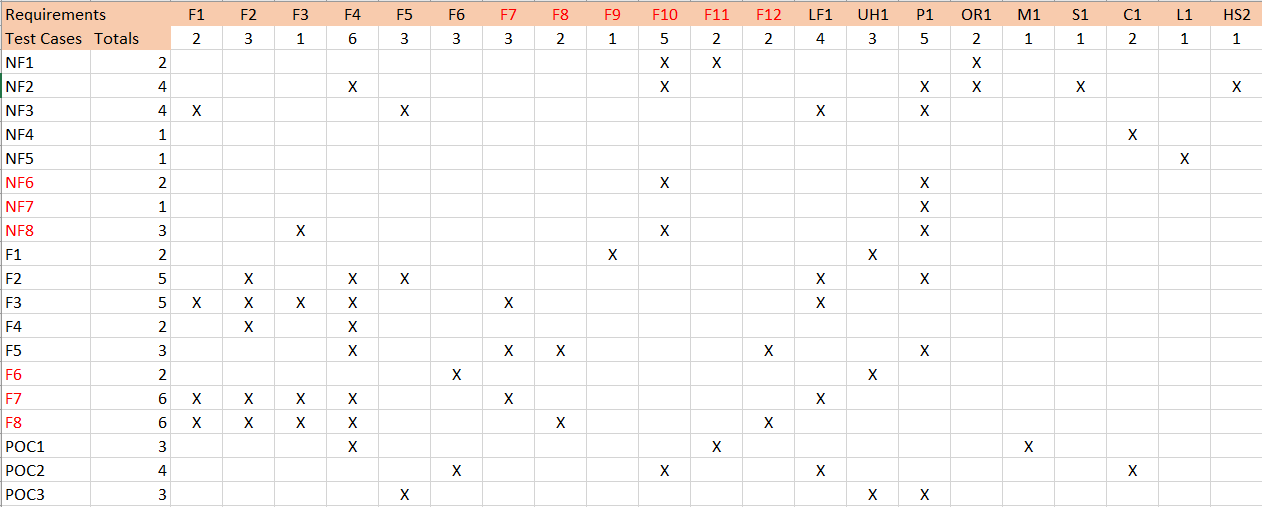
\includegraphics[width = 14cm, height = 6cm]{TraceabilityMatrix}
\caption{Traceability Matrix}
\end{figure}
		
		\newpage
\section{Trace to Modules}		
\noindent The following is the traceability matrix to modules defined in the Module Guide (Design Doc):
\begin{center}
\begin{table}[H]
\centering
\begin{tabular}{ |c| c| }\hline

 \textbf{Test Cases}    & \textbf{Modules}  \\ \hline
 F1   & M2, M3, M7, M11  \\ \hline
 F2   & M1, M7, M9  \\ \hline
 F3   & M4, M5, M7, M8, M9, M10, M11  \\ \hline
 F4   & M7, M8  \\ \hline
 F5   & M7, M9, M1, M10, M11  \\ \hline
 F6   & M4, M5, M7, M8  \\ \hline
 F7   & M7, M8, M9, M10  \\ \hline
 F8   & M5, M7, M8, M9  \\ \hline
 F9   & M1, M7, M8, M9  \\ \hline
 F10  & M3, M7, M11, M12  \\ \hline
 
 NF1  & M2, M3, M7  \\ \hline
 NF2  & M1, M3, M4, M5, M7, M8, M9, M10  \\ \hline
 NF3  & M7  \\ \hline
 NF4  & M3, M7, M10  \\ \hline
 NF5  & M7  \\ \hline
 NF6  & M1, M4, M5, M7, M8, M9, M11  \\ \hline
 NF7  & M3, M4, M5, M7, M8, M9, M10  \\ \hline
 NF8  & M1, M4, M5, M7, M8, M9  \\ \hline
 
 POC1 & M2, M7, M11, M12  \\ \hline
 POC2 & M3   \\ \hline
 POC3 & M1, M7  \\ \hline 
 
\end{tabular}
\caption{Trace Between Test Cases and Modules}
\end{table}
\end{center}


\section{Code Coverage Metrics}

Testing the Functional requirements the various tests were intended to explore almost all of the game's scripts in terms of running the game. These test were intended to encapsulate all of the various aspects of the game.\\

\textbf{Area of Testing 1:} This test ensured that the game button performed to their desired role, the test covered all of the levelManager script as well as the activation of some of the other scripts such as the high score in localLeader board, and hexagonBehaviour. \\

\textbf{Area of testing 2:} This test covers the collision and the behaviours of the trapzoid shapes with the hexagon. The test covers most of the trapzoidTransform scripts. \\

\textbf{Area of testing 3:} This test cover the rest of trapzoid transform in which area of testing 2 doesn't cover, this also covers the game scene.\\

\textbf{Area of testing 4:} This test covers the generation of the rapzoids at correct positions and at varied colors. It covers the code of trapzoidSpawner as well as the code for the various different trapzoids.\\

\textbf{Area of testing 5:} This test covers the block elimination of connected trapezoids ensuring that the flood fill algorithm is working correctly. Additionally it touches the collision code again for the trapezoids.\\

\textbf{Area of testing 6:} This test covers the game pause code and the stopping of some of the various functions such as the spawner as well as the button input. \\

\textbf{Area of testing 7:} This test case covers again the flood fill algorthim as well as the elimination of block. The rainbow trapezoid and its properties are covered as well. \\

\textbf{Area of testing 8:} This test case covers the blacktrapzoid code and its properties of being unable to be destryed matching with any other blocks except for rainbow blocks. \\

\textbf{Area of testing 9:} This test was again to run the trapzoid collision as well as the trapezoid behaviour and its properties and functionality with black trapezoids. Additionally it covers the player movement and the controls with the player Class.\\

\textbf{Area of testing 10:} This test is to test the conditions for gameOver stopping all game functions once 8 or more trapezoids are connected in a stack on any one side of the hexagon. \\

\noindent \textbf{Non-functional Testing:} \\

For these tests the specific amount of code coverage was less specific and more expansive as these test were intended to focus on the usability, robustness, and performance of the code which means that the code was take more as a whole.\\

\textbf{Non- Functional Area of testing 1:} Test to test the game start up code and loading of all the assets. \\

\textbf{
Non- Functional Area of testing 2:} This is a generate test to see the game under a continuous running of the program and all of its scripts. Here the test is expected to attempt to try all the features of the game covering all the code.\\

\textbf{Non- Functional Area of testing 3:} This test overviews the movement of the visuals of the game, it tests all the drawing sections of code from trapezoid, to player, to menus.
\textbf{Non- Functional Area of testing 4:} This test was not implemented to test much of the physical code but rather the various imagery used in the game, it does however touch the code which draws the images. \\

\textbf{Non- Functional Area of testing 5:} This test also was not meant focus on testing code but rather ensuring that all tasks have been in accordance with all legal rights. This test does ensure the code loading the text for the credits page are working.\\

\textbf{Non- Functional Area of testing 6:} This test covers almost every single line of code within the game as it was testing the smoothness of the game under all of its functions. From playing the game, to checking scores, to reaching game over, this test was to ensure all of the code run together and don't affect each other when all working in conjunction. \\

\textbf{Non- Functional Area of testing 7:} This test again was to test the impact of Hextron on the computer that is running it. The code that was covered is all of the code that run when the game is on the start screen.\\

\textbf{Non -Functional Area of testing 8:} This test was check the reliability of the Hextron program by opening multiple instance as well as multiple other programs all concurrently. This was to check to see if any outside program has effects affecting the program. Or if putting more pressure on the code (running multiple instances) will cause any problems. Again this test essentially ran through all the different functions and scripts of the Hextron program as one of the instances was played during the test. \\



\bibliographystyle{plainnat}

\bibliography{SRS}

\end{document}